\documentclass[twoside]{EPURapport}

\usepackage[utf8x]{inputenc}
\usepackage{amsmath}
\usepackage{graphicx}
\usepackage[colorinlistoftodos]{todonotes}
\nolistoftables

\thedocument{Rapport projet d'option RV}{Version 3D webgl de l'emploi du temps}

\grade{D\'epartement Informatique\\ 5\`eme ann\'ee \\ 2013 - 2014}
%\entitylogo{logos/spin_logo.PNG}

\authors{%
	\category{Étudiants}{%
		\name{Ping XIANG}
        \mail{ping.xiang@etu.univ-tours.fr}
        \name{Lei SHANG}
        \mail{lei.shang@etu.univ-tours.fr}
	}
	\details{DI5 2013 - 2014}
}

\supervisors{%
	\category{Encadrants}{%
		\name{Sébastien Aupetit} 
        \mail{sebastien.aupetit@univ-tours.fr}
	}
	\details{École polytechnique de l’université de Tours Tours - FRANCE}
}

\abstracts{Ce rapport est rédigé à la suite d'un projet d'option Réalité Virtuelle. Dans le projet nous avons réalisé une application qui peut afficher l'emploi du temps d'un étudiant DI sur le modèle 3D du bâtiment. L'application peut aider les nouveaux étudiants à trouver une salle et même le plus court chemin entre deux salles. Une animation de navigation peut aussi lancer le long du chemin pour guider l'utilisateur.}
{Réalité virtuelle, Emploi du temps 3D, Plus court chemin, Three.js, Plugin Chrome}
{This report is edited for a project in the option Réalité Virtuelle. In this project we have implemented an application which can show students' class schedule on the 3D model of our teaching building DI. It helps new students to find easily the position of classrooms and even the shortest path from one room to anther. A guiding tour animation along the path can be launched as well.}
{Virtual reality, 3D class timetable, Shortest path, Three.js, Chrome plugin}



\begin{document}
\title{EDT3D}

\chapter{Introduction}
Ce rapport est développé à la suite du projet d'option Réalité Virtuelle: Version 3D WebGL de l'emploi du temps. L'objectif du projet est de visualiser en 3D notre emploi du temps des cours en l'affichant directement sur le modèle 3D de notre département, pour rendre ces informations plus représentatives.

\bigskip

Plus précisément, les fonctionnalités à réaliser sont:
\begin{enumerate}
	\item Modélisation du bâtiment DI en modèle 3D
    \item Importation de l'emploi du temps à partir d'un fichier ICS
    \item Importation de l'emploi du temps directement depuis l'ENT
    \item Analyse et extraction des données de l'emploi du temps
    \item Visualisation des cours sur la scène 3D
    \item Affichage du plus court chemin entre 2 salles
\end{enumerate}

\bigskip

Ce projet est réalisé avec les technologies web notamment webGL de manière à être utilisable depuis un navigateur. Toutes les fonctionnalités ci-dessus ont été réalisées sauf l'importation de l'emploi du temps depuis l'ENT. Ceci est prouvé infaisable à cause de la manque de l'information sur le format des données échangées. Par contre l'utilisateur peut très bien exporter sois même son emploi du temps et fournir l'URL exportée à l'application. Nous avons donc réalisé cette fonctionnalité de substitution.

\bigskip

En plus, nous avons réalisé des fonctionnalités supplémentaires pour rendre notre application encore plus conviviale, voici une liste non-exhaustive:
\begin{enumerate}
	\item Recherche de la position des salles
    \item Calcule et affichage du plus court chemin entre 2 salles choisies
    \item Animation de la caméra le long le chemin pour une navigation guidée
    \item Affichage des informations des cours en texte
    \item Mise en ligne de notre site web
    \item Création d'un plugin Chrome de l'application dans \textit{Google Web Store}
\end{enumerate}

\bigskip

Dans la partie suivante, nous allons expliquer en détail ce que nous avons réaslié ainsi que les difficultés rencontrées.


%%%%%%%%%%%%%%%%%%%%%%%%%%
%%%  Travaux réalisés %%%%
%%%%%%%%%%%%%%%%%%%%%%%%%%
\chapter{Travaux réalisés}
%\section{Technologies employées}
%\subsection{three.js}
%\subsection{jQuery}   时间有限我看这个可以不介绍。
%\subsection{bootstrap}

%%%%%%%%%%%%%%%%%% Modèlisation %%%%%%%%%%%%%%%%%%%%
\section{Modèlisation 3D du bâtiment}  
Dans cette section, nous présentons les travaux sur la mesure et la modélisation des composants du bâtiment comme les salles, les étages, les escaliers, et les points de contrôle pour calculer le plus court chemin.  

\subsection{three.js}
Three.js est une bibliothèque JavaScript graphique 3D, elle est basée sur WebGL qui fournit <canvas>, <svg>, CSS3D et WebGL rendus. Nous l'utilisons pour modéliser notre bâtiment.

\subsection{Mesure et collection des données de la modélisation}

\subsubsection{Mesure les coordonnées}

Pour modéliser les composants, tout d'abord, on a besoin de les mesurer précisément. Nous avons trouvé les plans de chaque étage du bâtiment de l'école, puis nous avons choisi le coin en bas à gauche comme l'origine. Nous avons utilisé une règle pour mesurer la coordonnée de chaque composant en centimètres. Ensuite, nous les avons converties en pixels et calculé la longueur et la largeur de chaque salle.

La figure \ref{fig:mesure} est pour donner une idée sur notre travail est n'est pas difficile mais qui est coûteux au niveau du temps dépensé.

	\begin{figure}[!htbp]
	\centering
		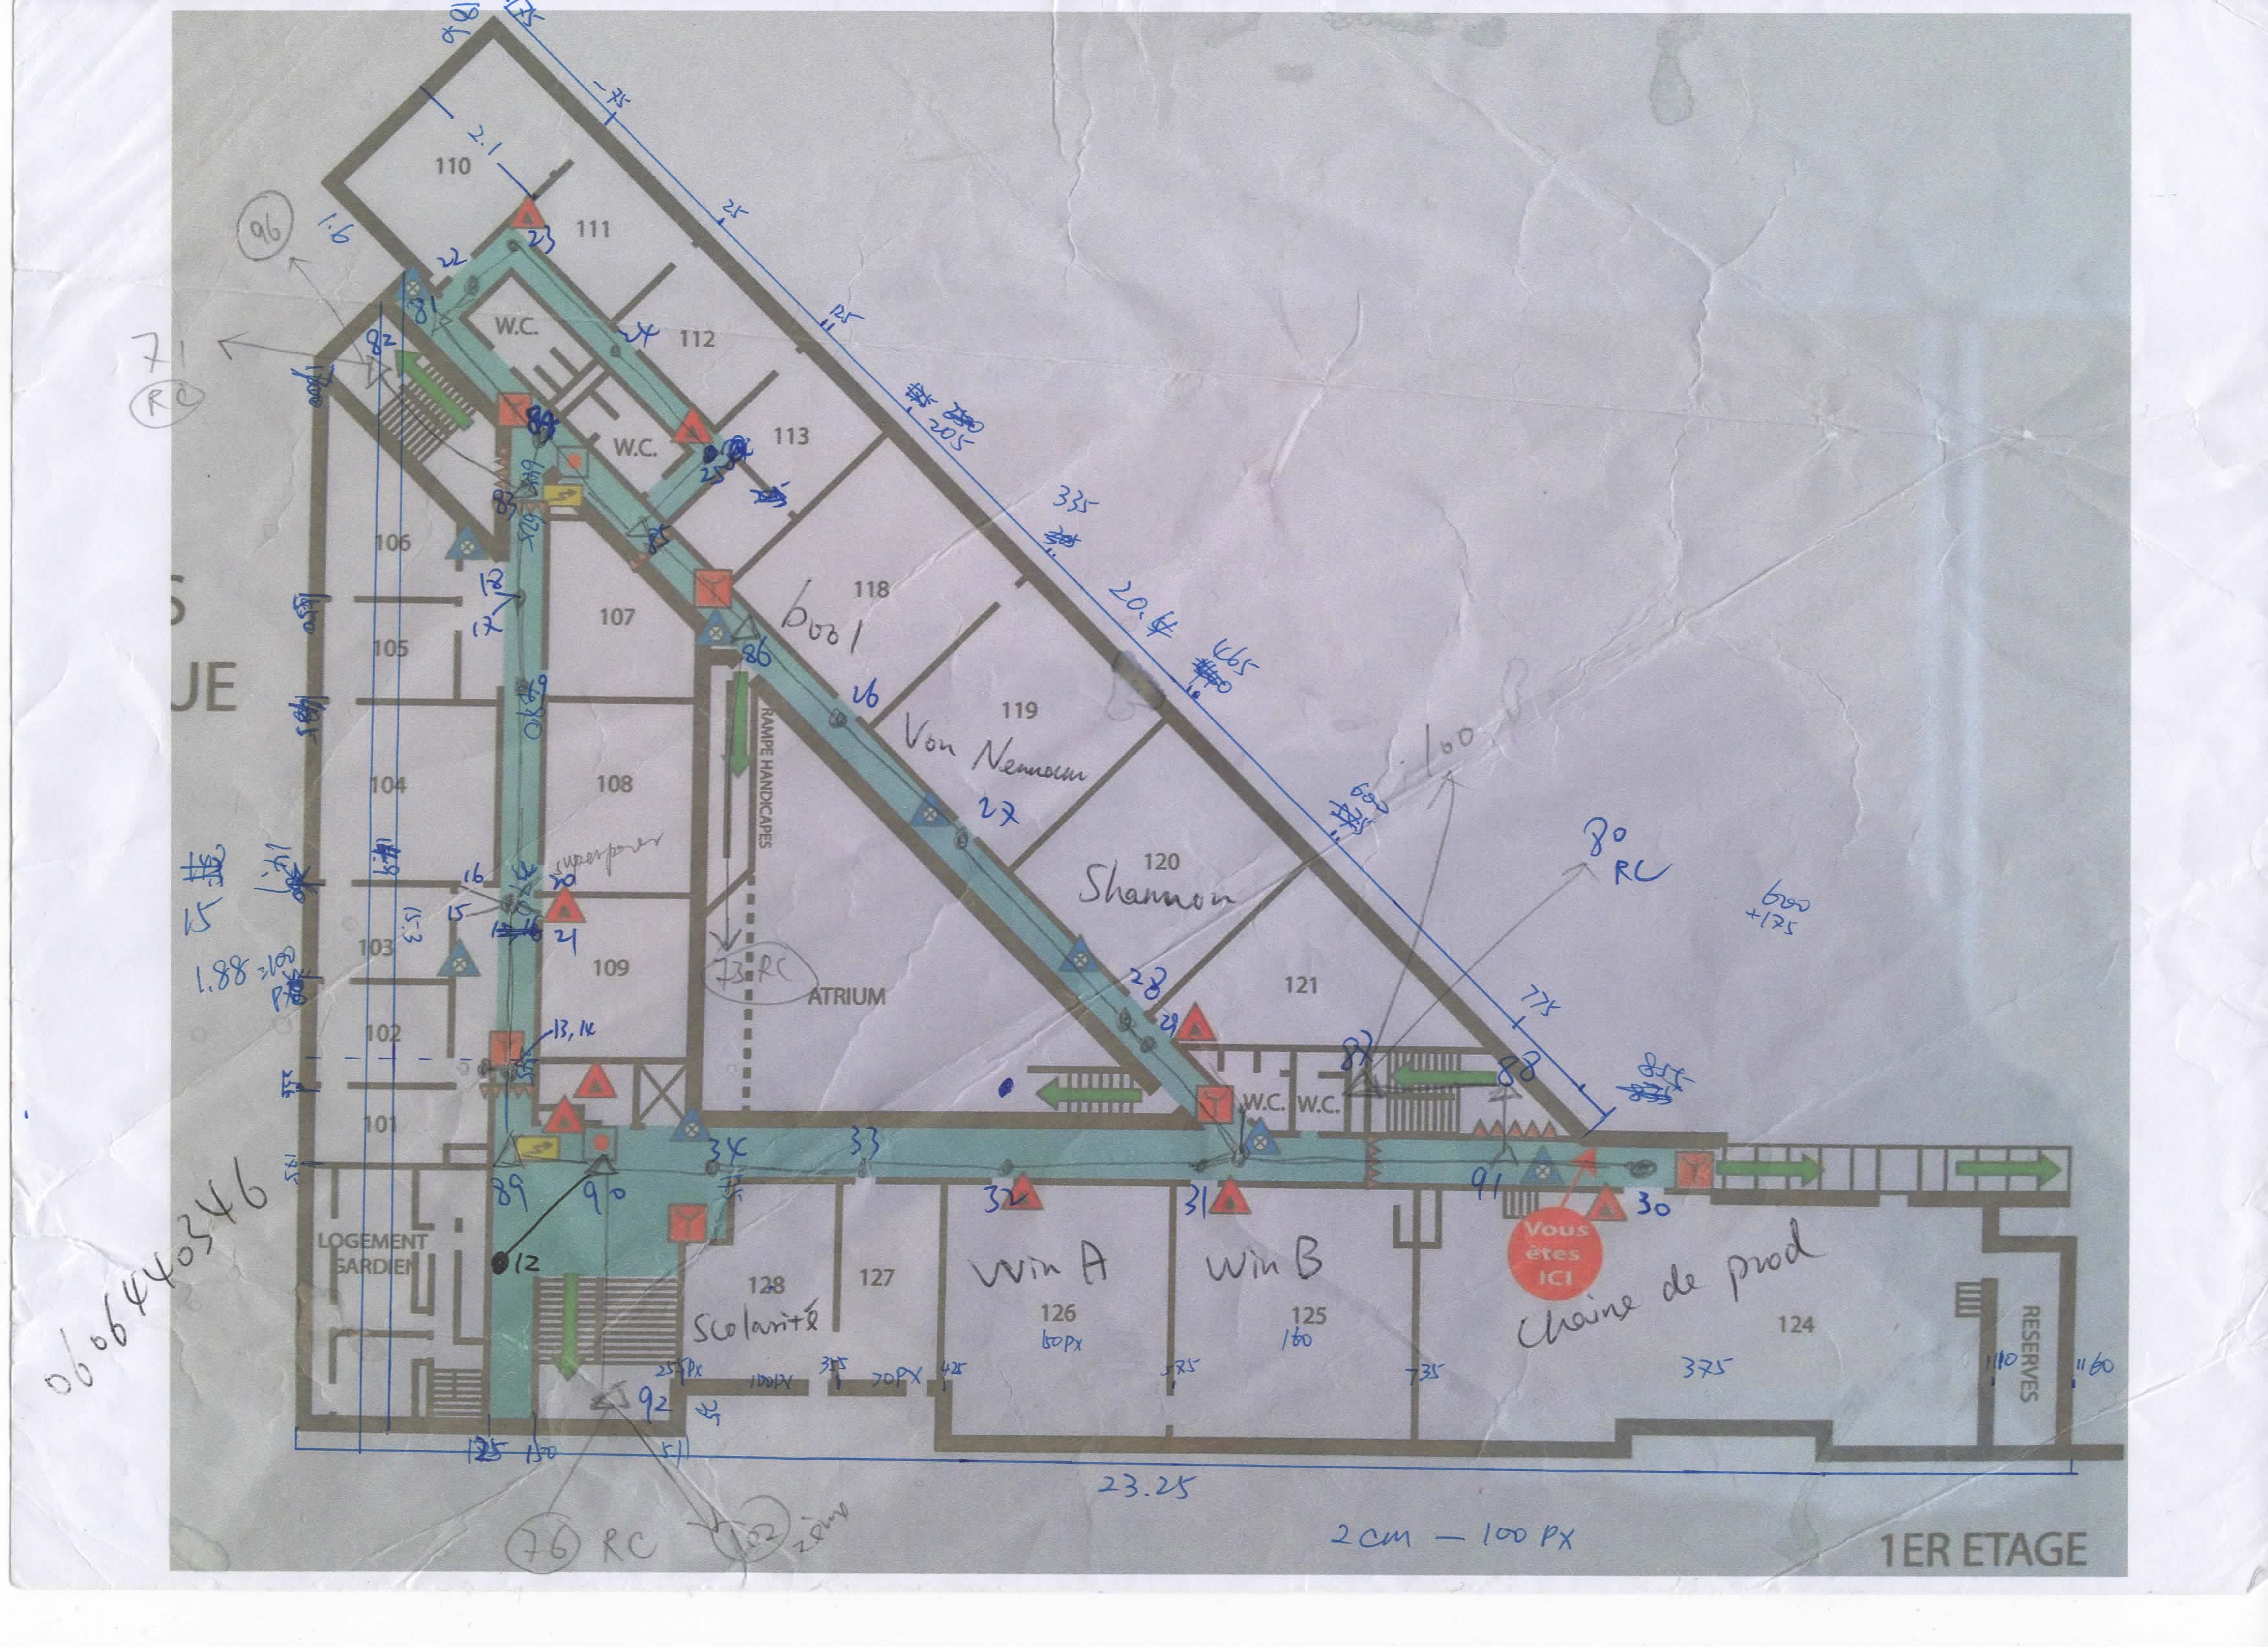
\includegraphics[scale=0.45]{img/mesure.jpg}
	\caption{La mesure des coordonnées}
	\label{fig:mesure}
	\end{figure}

\subsubsection{Stockage des coordonnées}
Nous définissons une structure de données pour représenter chaque composant. Les différentes structures qui contiennent des informations nécessaires pour modéliser un composant sont les suivantes :

\paragraph{Salle}

\begin{itemize}
	\item id, identifiant de salles, de 0 à 61.
    \item numéro, un nombre qui représente le numéro de la salle
   	\item nom, le nom des salles définies par l'école. Il va être apparu sur les murs des salles, et être utilisé pour trouver une salle.
    \item position, la coordonnée du point du centre de salle.
    \item taille, un vecteur contient la longueur, la largeur, et la hauteur. La hauteur est définie par nous.  
    \item format, les salles de l'école disposent de deux formes, carré et trapézoïdale. Pour les salles carrées, nous pouvons dessiner directement une géométrie de cube; et pour les salles trapézoïdales, selon la position et la taille, nous pouvons calculer les coordonnées de chaque vertex, et dessiner 2 triangles par face, au total 12 triangles constituants une trapézoïdale.
    
    \begin{figure}[!htbp]
	\centering
		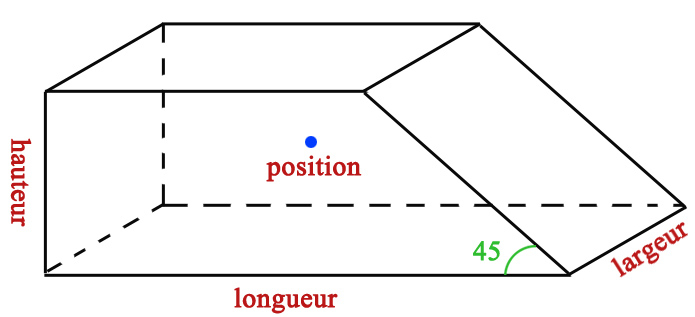
\includegraphics[scale=0.4]{img/trapezoidale.jpg}
	\caption{Une salle trapézoïdale}
	\label{fig:salle}
	\end{figure}
    
    \item direction, les salles de l'école ont 3 directions: horizontale, verticale et oblique. Après la création des salles, nous faisons la rotation pour les faire correspondre la direction donnée. 
\end{itemize}

\paragraph{Etage et escalier}
Les étages et escaliers sont construits par des faces. Nous mesurons et fixons les vertex des faces, et choisissons le matériel.

\paragraph{Points clés pour calculer le plus court chemin}

\begin{itemize}
	\item id, un nombre unique utilisé pour identifier les points. De 0 à 61, les points sont positionnés dans les couloirs devant les salles; de 70 à 103, les points supplémentaires placés sur les escaliers, tournant, entrée, etc, utilisés pour garantir la naturalité du chemin. Par exemple, on ne doit pas laisser le chemin traverser un mur. 
    \item position, les coordonnées des points.
    \item direction, le même sens que pour les salles.
\end{itemize}

\subsection{Conception de la scène}
Lorsque ce projet a été proposé, nous espérons que nous pouvons montrer les locations des cours plus clairement, pour guider les étudiants à trouver rapidement l'emplacement de la classe. Par conséquent, nous avons décidé les choses suivantes afin de répondre à notre concept :

\begin{itemize}
\item utiliser une couleur claire pour les salles,;
\item utiliser les couleurs suivantes pour distinguer les salles en les différents états (figure \ref{fig:color}):
	\begin{itemize}
	\item rouge, représente la salle recherchée
    \item vert, représente la salle du prochain cours
    \item bleu, représente la salle en cours en ce moment
    \item gris foncé, représente la salle dont le cours a déjà fini
	\end{itemize}

\item afficher le nom des salles sur le mur de chacune pour montrer plus clairement les positions;

\item ajouter le sol du premier étage pour éviter le chevauchement excessif de salle;

\item L'élargissement de la position des escaliers pour fournir une meilleure perspective.

\end{itemize}

\begin{figure}[!htbp]
	\centering
		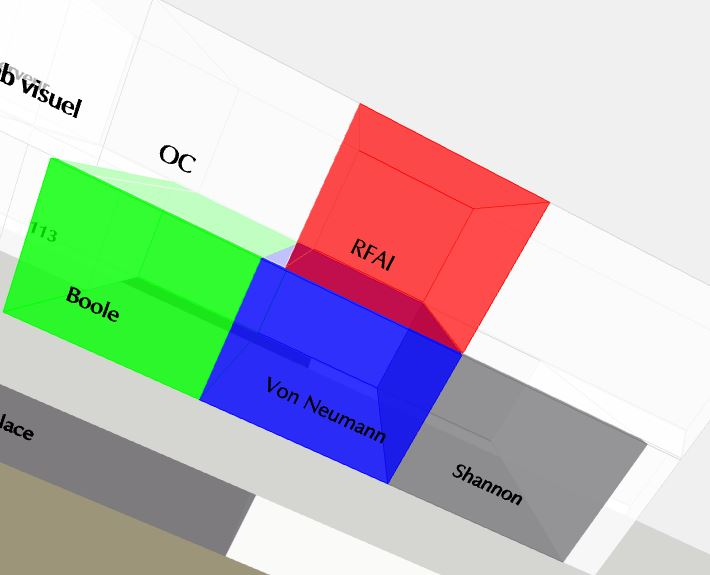
\includegraphics[scale=0.6]{img/stats.JPG}
	\caption{Les salles en différents états}
	\label{fig:color} 
\end{figure}
\bigskip

\subsection{Difficultés rencontrées}

% three.js 文档不详细,时常需要查找实例和代码。%建模很耗精力
Le premier problème rencontré est que la création du modèle de l'école est très chronophage. Nous devons mesurer chaque salle précisément afin de modéliser plus réellement le modèle 3D, nous avons dépensé beaucoup de temps sur celui-ci. En même temps, la documentation de three.js n'est pas très précise. Pour de nombreuses classes et fonctions, il n'y a pas de documentation, ni d'exemple, nous étions souvent obligés d'entrer dans le code source pour nous débrouiller.


%%%%%%%%%%%%%%%%% Traitement des données %%%%%%%%%%%%%%%%%%%
\section{Traitement des données de l'emploi du temps}
Dans cette partie nous présentons le travail sur la récupération et l'analyse des données de l'emploi du temps. Les informations extraites des cours seront intégrées dans le modèle 3D de notre bâtiment pour enfin montrer à l'utilisateur.
\subsection{Récupération de l'emploi du temps}
Les données des cours de l'école se présentent sur le site ENT\footnote{Environnement Numérique de Travail, \url{http://edt.univ-tours.fr/direct/myplanning.jsp?login=ade-etudiant&password=test}} de l'université. 

\begin{figure}[!htbp]
	\centering
		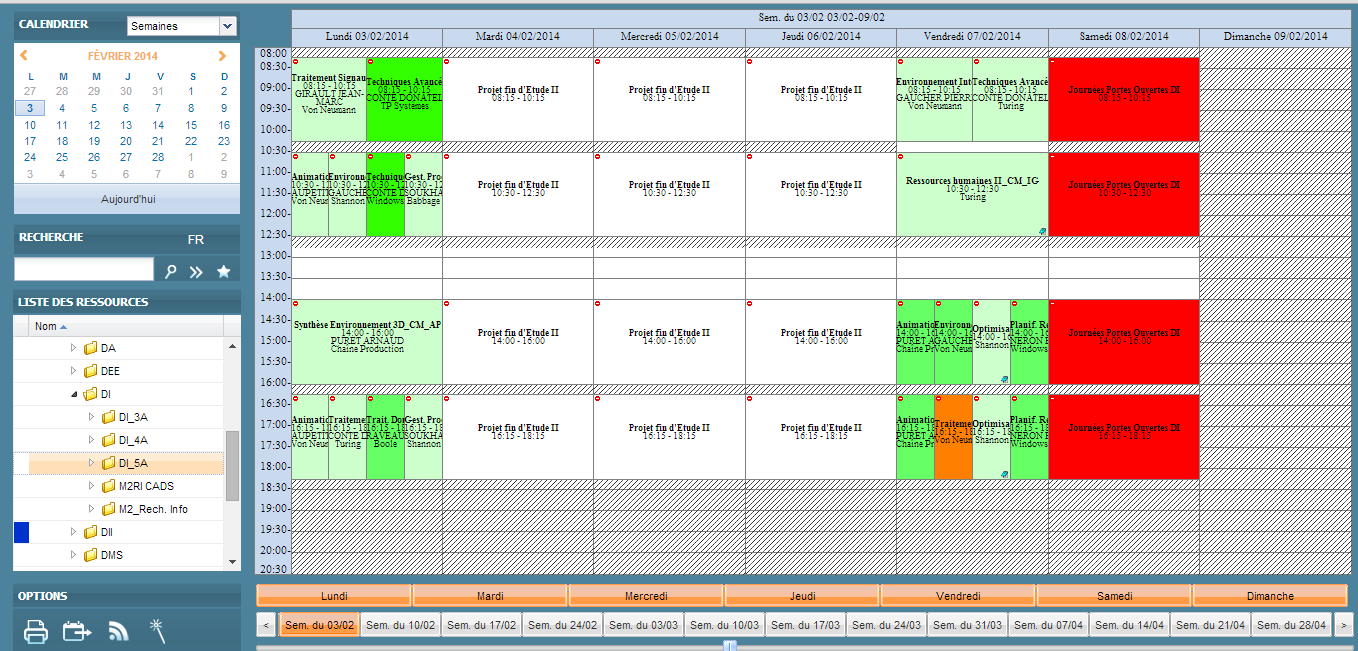
\includegraphics[scale=0.5]{img/ent.png}
	\caption{ENT}
	\label{fig:ent} 
\end{figure}
\bigskip

\subsubsection{Récupération directe à partir de l'ENT} %%%%%
Le site ENT est une application web assez lourde qui regroupe les services informatiques de tous les étudiants de l'université. La récupération de l'emploi du temps à partir de cette application n'est pas évidente.


Dans un premier temps nous avons analysé le flux transféré entre le site ENT et le navigateur pour trouver comment les données de l'emploi de temps sont transférées. Nous avons enfin trouvé des morceaux de ces informations dans plusieurs tableaux json qui contiennent chacun énormément d'enregistrements. En fait, ce qui est transmis n'est pas seulement les données de l'emploi du temps, mais aussi un grand volume de données d'ailleurs, puisque c'est une page web riche.

La figure\ref{fig:ent_requestheader} est la requête que nous avons captée, qui est envoyée par le navigateur pour demander les données. La méthode d'envoi est \textit{POST}, le charge de la requête contient beaucoup de chiffres dont nous ne comprenons pas le sens.
\begin{figure}[!htbp]
	\centering
		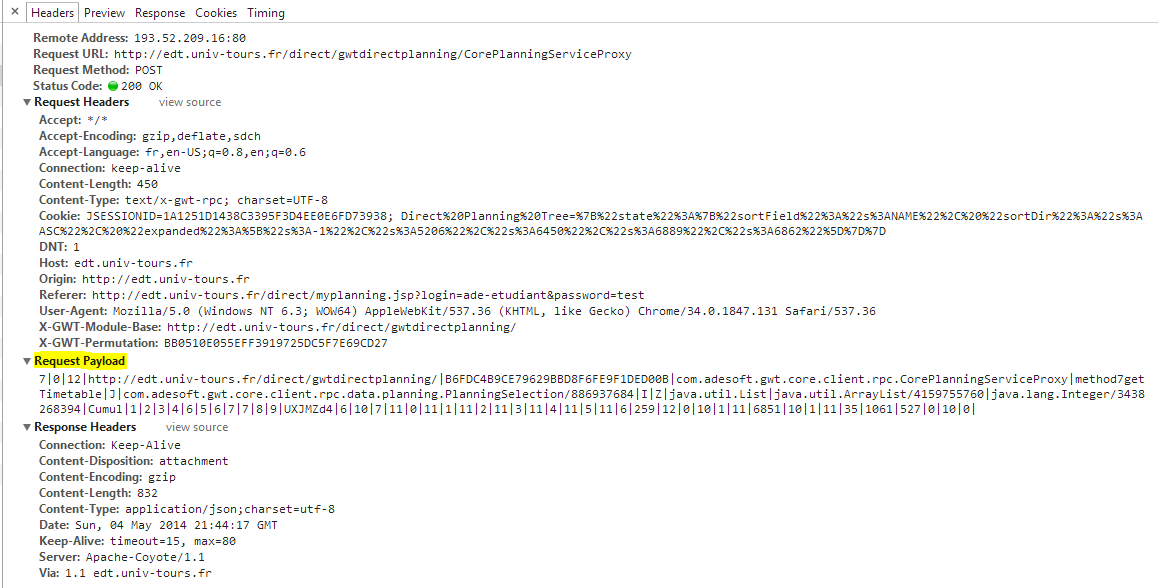
\includegraphics[scale=0.6]{img/ent_requestheader2.png}
	\caption{La requête envoyée depuis le navigateur}
	\label{fig:ent_requestheader} 
\end{figure}
\bigskip

La figure\ref{fig:ent_response} est la reponse du serveur. Il y a plein de chiffres encodés. Même si nous avons trouvé des morceaux de données qui nous intéresse, nous n'avons pas pu trouver un moyen pour extraire ces données en analysant la réponse du serveur car il n'y a pas assez d'information. L'extraction directe de l'emploi du temps à partir de l'ENT devient donc infaisable pour nous. Nous avons ensuit basculer à d'autres méthodes de récupération.
\begin{figure}[!htbp]
	\centering
		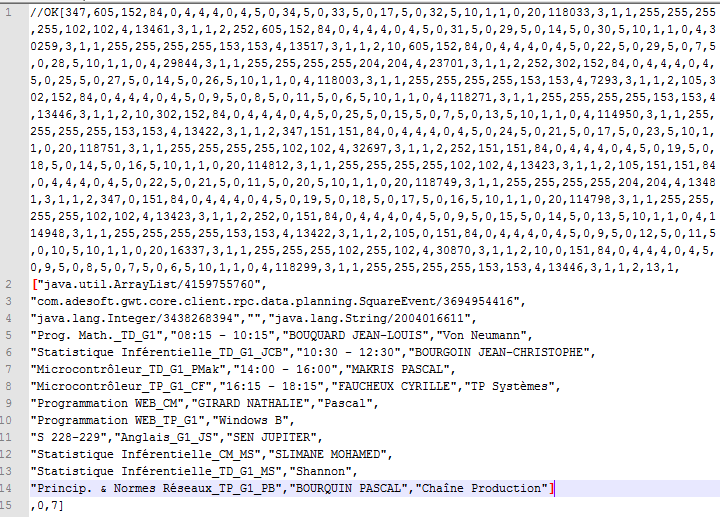
\includegraphics[scale=0.7]{img/ent_response.png}
	\caption{La réponse reçue qui contient les données de l'emploi du temps}
	\label{fig:ent_response} 
\end{figure}
\bigskip


\subsubsection{Récupération des données par URL d'exportation}%%%%%
Nous avons constaté que l'ENT fournit l'exportation de l'emploi du temps en URL. On doit d'abord choisir sa spécialité puis la période à exporter. En sortie on obtiendra une URL à partir duquel un fichier ICS\footnote{\href{http://fr.wikipedia.org/wiki/ICalendar}{ICalendar, standard RFC 5545}} qui contient les informations des cours peut être téléchargé.


Nous avions utilisé ce moyen pour exporter l'emploi du temps dans notre propre calendrier comme Google Agenda, donc nous pensons que c'est possible que nous fassions la même chose, c'est-à-dire récupérer les données depuis une URL d'exportation.

\begin{figure}[!htbp]
	\centering
		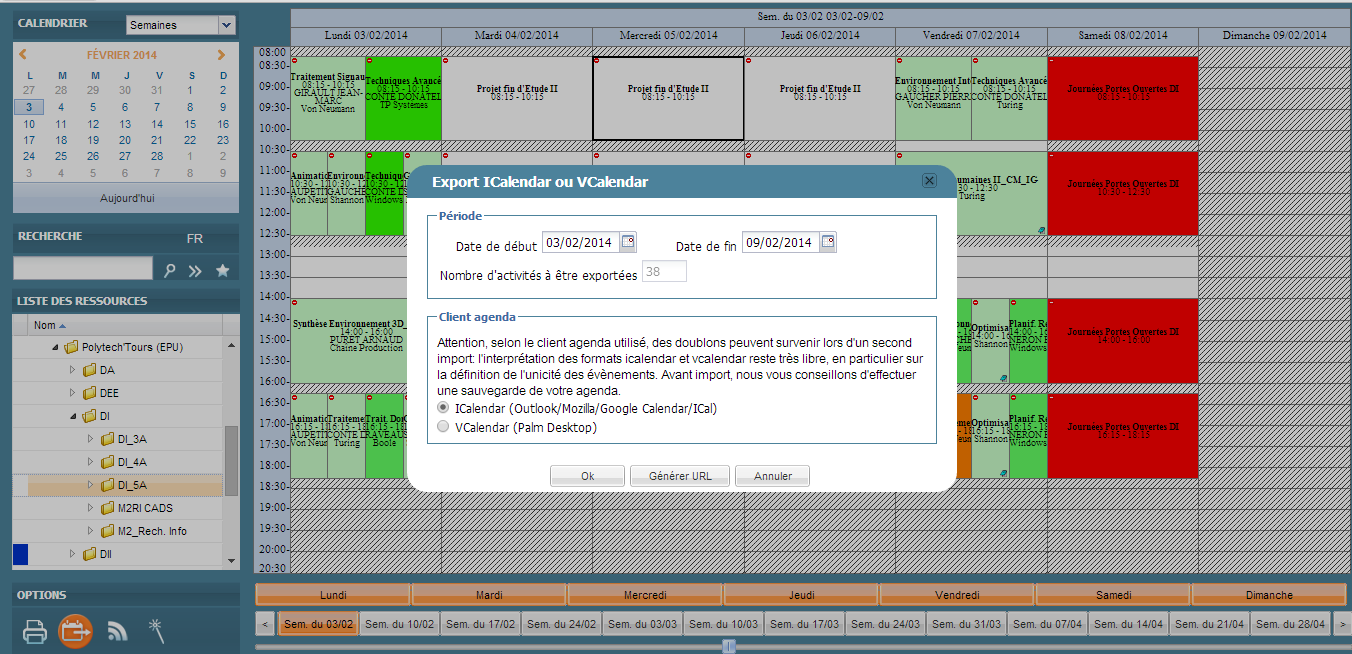
\includegraphics[scale=0.4]{img/export.png}
	\caption{Exportation du calendrier en URL}
	\label{fig:export}
\end{figure}
\bigskip

\begin{figure}[!htbp]
	\centering
		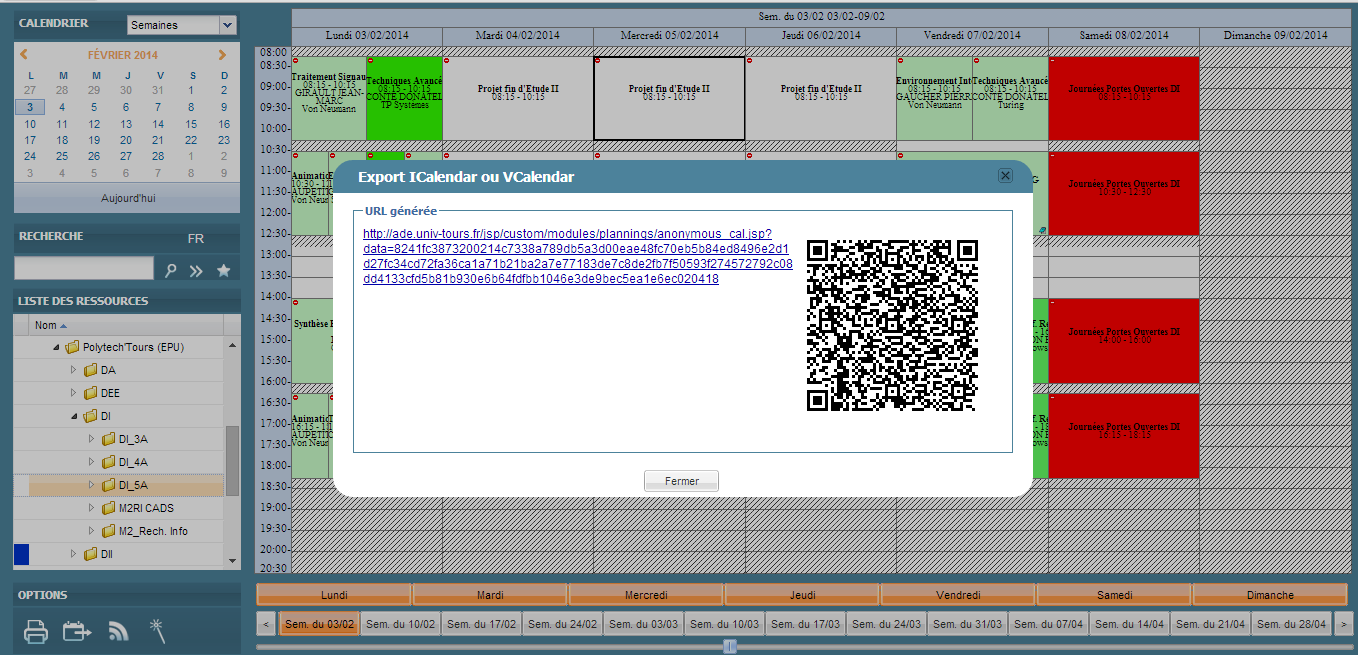
\includegraphics[scale=0.4]{img/url.png}
	\caption{URL d'exportation générée}
	\label{fig:url}
\end{figure}
\bigskip

Pour le faire, nous demandons l'utilisateur de générer d'abord cette URL sur l'ENT et puis le fournir à notre application pour la première utilisation. Nous allons ensuite enregistrer cette URL et synchroniser l'emploi du temps à chaque ouverture de l'application.


Nous avons rencontré des difficultés pour le téléchargement du fichier ICS. Ce sera expliqué dans la section difficultés rencontrées\ref{sec_diff}.

\subsection{Analyse et extraction des cours}%%%%
Après l'obtention des données de format ICS, il nous reste à analyser ces données et d'extraire les cours selon la date choisit. Nous avons d'abord étudié le format ICS, ensuite nous avons créé des expressions régulières qui nous permettent de trouver et extraire les informations qui nous intéressent. 


Ce travail a été réalisé avec JavaScript, en sortie de cette analyse on a un tableau des événements (cours) qui sont des objets avec les attributs comme: l'horaire du cours, le nom et le lieu du cours, etc. Ces objets seront intégrés après dans le modèle 3D.


\subsection{Difficultés rencontrées}\label{sec_diff} % 由于安全性问题无法直接使用网页,于是创建了plugin 甚至 PHP后台
La principale difficulté dans cette partie de travail concerne la récupération directe des données depuis l'ENT. Nous avons mis beaucoup de temps pour chercher un moyen, mais finalement nous n'avons pas réussi.


La récupération depuis URL d'exportation nous a posé aussi des problèmes. En fait nous avons voulu au tout début, de rendre notre application web purement locale, c'est-à-dire tout le travail de notre application serait réalisé par JavaScript donc pas besoin de mettre en place un serveur. Malheureusement le comportement du téléchargement \textit{cross-domain} de données n'est pas autorisé par défaut par des navigateurs (Chrome pour nous) à cause des soucis de sécurité. Souvent nous pouvons demander le navigateur à l'autoriser en modifiant l'option concernée, mais ça rend notre application beaucoup moins conviviale et surtout ça va exposer nos chers utilisateurs sous danger.


Finalement nous étions obligés de créer la côte serveur en PHP de l'application, pour évider un téléchargement \textit{cross-domain}. En plus, pour donner plus de choix et de meilleures expériences aux clients, sans jamais oublier notre rêve de \textit{localisation}, nous avons aussi créé un plugin Chrome\footnote{Les applications Chrome peuvent avoir des droits supplémentaires comme la requête cross-domain dans notre cas} de l'application qui est déjà mis en ligne dans \textit{Chrome Web Store}.%\footnote{\url{}https://chrome.google.com/webstore/detail/edt3d/deidljgkpcpmknnbcempgmnljjmdodlb?hl=fr}.

%%%%%%%%%%%%%%%%%%%
\section{Plus court chemin}
La recherche du plus court chemin est un problème très classique, mais toujours intéressant. Dans ce projet nous avons pu appliquer l'algorithme \textit{Dijkstra} pour chercher le plus court chemin entre 2 salles de l'école. %Le code source en JavaScript peut être trouvé dans l'Annexe\ref{annexe}.


Notre idée est de positionner dans le modèle des points clés qui sont des noeuds du graphe, pour afficher le chemin, nous pouvons donc relier les points qui composent le chemin.

\subsection{Implémentation de l'algorithme Dijkstra}	%%%%%
Pour appliquer l'algorithme de la recherche du plus court chemin, il faut d'abord modéliser notre problème en une structure de graphe en JavaScript. Nous avons alors créé une class \textit{Graphe} qui peut représenter un graphe et qui contient des méthodes nécessaires pour la création du graphe.


Après étudier la particularité de notre problème et l'algorithme Dijkstra, nous avons choisi de stocker les noeuds dans une liste et pour chaque noeud nous maintenons une liste des noeuds voisins. De cette manière, l'implémentation de l'algorithme devient plus simple et sa performance peut être garantie.


Finalement le graphe de notre bâtiment contient centaine sommets, ce qui est un graphe plus grand que prévu.

\subsection{Affichage et animation du chemin} %%%%%
\subsubsection{Affichage}
A chaque fois l'emploi du temps se charge, l'application va chercher, selon l'horaire en ce moment, le cours suivant à assister. Ensuite elle applique l'algorithme pour trouver le plus court chemin entre la salle du cours en cours (ou le point d'entrée s'il n'y a pas de cours en ce moment) et la salle du cours suivant. Ce chemin est représenté d'un tableaux des indices des points clés. Nous créons ensuite à l'aide de \textit{three.js}, un \textit{SplineCurve} basé sur ces points clés et puis un \textit{TubeGeometry} qui est le chemin fininal.


Pour bien afficher le chemin, il y a énormément de points à positionner: à part des points devant chaque salle, il faut aussi ajouter des points intermédiaires pour assurer que le chemin est bien \textit{naturel}, par exemple il faut mettre des points sur les tournants pour que le chemin ne traverse pas le mur.


\begin{figure}[!htbp]
	\centering
		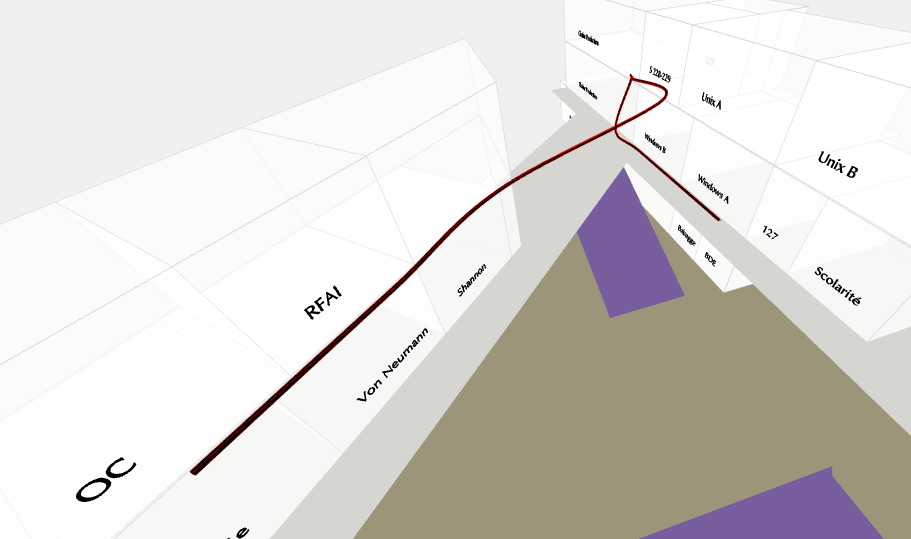
\includegraphics[scale=0.5]{img/oc_wina.png}
	\caption{Le plus court chemin de la salle OC à Windows A : affichage}
	\label{fig:oc_wina}
\end{figure}
\bigskip

\subsubsection{Animation}
Puisque notre bâtiment est de forme d'un triangle, ce qui est un peu fermé pour avoir une bonne vue du chemin affiché. Nous pensons donc de \textit{"guider"} l'utilisateur le long du chemin, c'est-à-dire d'animer la caméra pour qu'il se déplace le long du chemin. Nous avons aussi affiché en 3D le numéro des salles à côté du chemin, donc pendant le parcours on peut toujours se percevoir sa position dans le bâtiment. (cf Figure\ref{fig:oc_wina_anim})

\begin{figure}[!htbp]
	\centering
		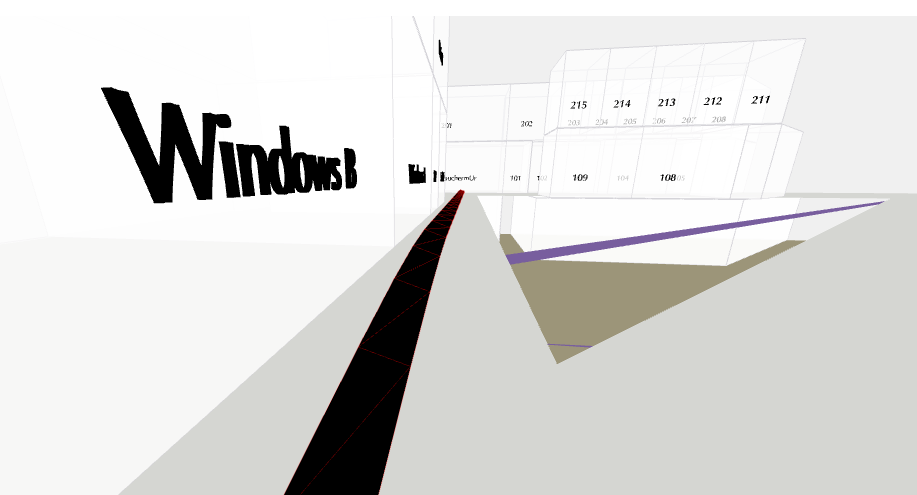
\includegraphics[scale=0.5]{img/oc_wina_anim.png}
	\caption{Le plus court chemin de la salle OC à Windows A : animation de la caméra}
	\label{fig:oc_wina_anim}
\end{figure}
\bigskip


%%%%%%%%%%%%%%%%%%%
\section{Application créée} %界面截图。也可以放在最后
Afin de rendre mieux l'IHM du site, nous le divisons en deux parties avec l'étiquette iframe : la partie gauche est le panel de configuration, réalisé en utilisant bootstrap ; la partie droite affiche notre modèle 3D.



\subsection{IHM}
L'IHM de notre application contient deux parties: un panel de configuration à gauche et la vue 3D du bâtiment à droite.

\begin{figure}[!htbp]
	\centering
		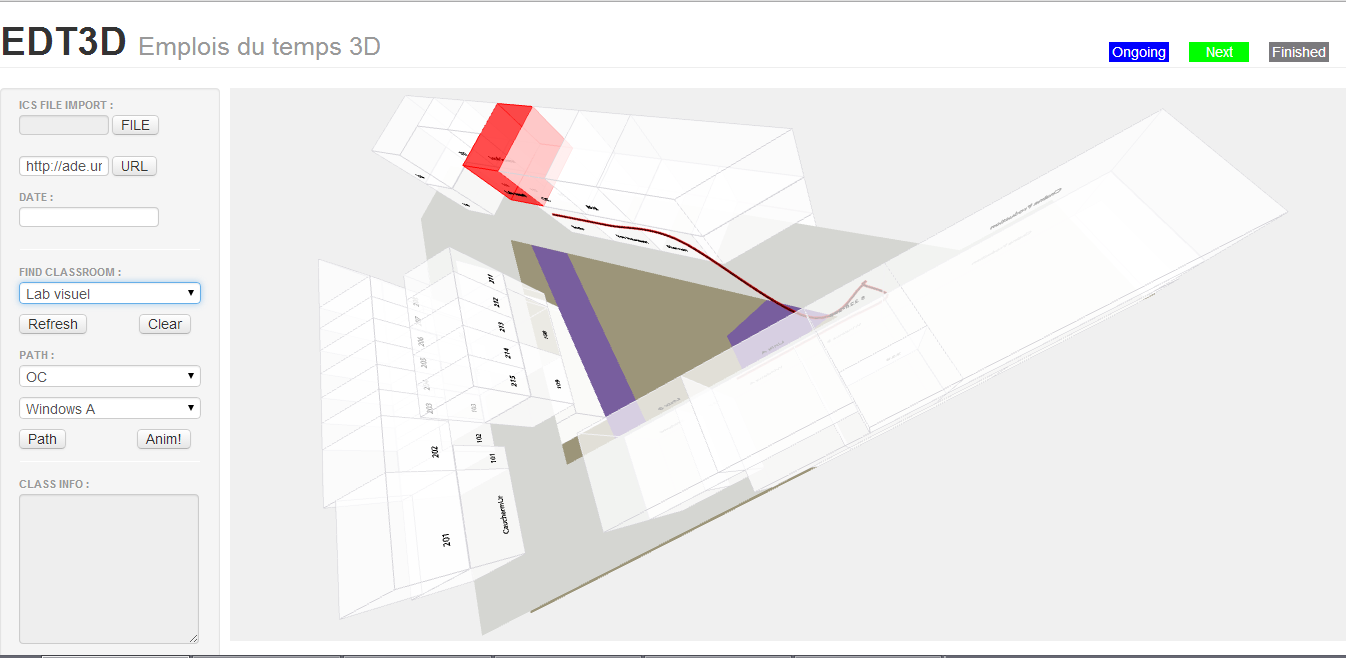
\includegraphics[scale=0.5]{img/ihm.png}
	\caption{L'IHM de l'application}
	\label{fig:ihm}
\end{figure}
\bigskip

\subsubsection{Panel de configuration}
Les fonctionnalités dans le panel à gauche sont:
\begin{itemize}
	\item \textbf{Choix du fichier ICS}: importation de l'emploi du temps depuis un fichier en format ics.
    \item \textbf{Saisie de l'URL ICS}: importation de l'emploi du temps depuis une URL.
    \item \textbf{Date}: après l'importation, ce champ sera activé qui permet de choisir une date dont les cours seront affichés dans la vue.
    \item \textbf{Recherche de salles}: pour trouver la position d'une salle, on peut choisir la salle dans la liste, elle sera indiquée dans le modèle 3D.
    \item \textbf{Path}: afficher le plus court chemin entre 2 salles choisies. Le bouton \textit{Path} permet de calculer et d'afficher le chemin, le bonton \textit{Anim!} va lancer l'animation de la caméra selon le chemin précalculé.
    \item \textbf{Classinfo}: afficher en texte les cours de la date choisie. La mise en place de ce champ est pour traiter le problème que pour certains cours la salle n'est pas indiquée dans l'emploi du temps, par exemple pour le \textit{Projet d'Option}. Dans ce cas-là, nous ne pouvons bien sûr pas afficher ce cours dans la vue 3D.
\end{itemize}

L'apparence de cette partie est créée à l'aide de Bootstrap qui est un cadre frontal élégant, intuitif et puissant pour le développement web rapide et plus facile. Il est créé par Mark Otto et Jacob Thornton, et maintenu par l'équipe de base avec le soutien massif et la participation de la communauté.

\subsubsection{Navigation dans la vue 3D}
Pour naviguer dans la vue 3D:
\begin{itemize}
	\item \textbf{Rotation}: trainer avec le bouton gauche de la souris.
    \item \textbf{Translation}: trainer avec le bouton droit de la souris.
    \item \textbf{Zoom}: la molette de la souris.
\end{itemize}


\subsection{Publication de l'application}
Grâce à la difficulté rencontrée\ref{sec_diff} pendant la récupération des données, nous avons enfin créé trois versions de notre application.

\subsubsection{Application web serveur}
Cette version est une application web en PHP. Il faut la mettre sur un serveur pour être accessible par les utilisateurs. Pour rendre notre projet \textit{complet}, nous avons mis en ligne notre application. Elle est accessible depuis cette URL: \url{http://edt3d.site40.net/}, mais l'accessibilité ne sera pas toujours garantie.

\subsubsection{Application Chrome}
Cette version est un plugin Chrome qui peut être installé directement dans le navigateur Chrome par les utilisateurs. Ce plugin est déjà mise dans le \textit{Chrome Web Store} d'où tout le monde peut le télécharger\url{https://chrome.google.com/webstore/detail/edt3d/deidljgkpcpmknnbcempgmnljjmdodlb?hl=fr}. Une icône de l'application apparaîtra dans la barre des plugins.
\begin{figure}[!htbp]
	\centering
		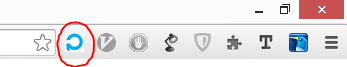
\includegraphics[scale=1]{img/plugin.png}
	\caption{Plugin Chrome}
	\label{fig:plugin}
\end{figure}
\bigskip

\subsubsection{Application web locale}
Cette version est la version initiale qui a posé le problème de sécurité. Mais à part de ce risque, c'est quand même une version utilisable donc tout dépend le choix de clients.

%%%%%%%%%%%%%%%%%%%%%%%%%%%%%
%%%%%%% Conclusion  %%%%%%%%%
%%%%%%%%%%%%%%%%%%%%%%%%%%%%%
\chapter{Conclusion}
Ce projet nous a permis de pratiquer les techniques de Réalité Virtuelle sur un problème réel. L'application que nous avons créée peut aider les nouveaux étudiants à facilement trouver la position des salles et même le plus court chemin pour assister un cours. C'est très pratique et très proche de notre vie, donc ça nous fait sentir que notre travail et les techniques 3D que nous avons appris ont de la valeur.


Au niveau technique, nous avons pu bien connaître un outil JavaScript de développement 3D: \textit{three.js}, nous avons aussi maîtrisé le développement de plugin Chrome.


En un mot, ce projet nous a beaucoup plu et nous a renforcé les connaissances sur la réalité virtuelle.
\end{document}
